
\label{cha:res}
% \section{Verdunstungsexperiment}
% \label{res:eva}
% 
% \subsection{Präsentation}
% \label{res:eva:pres}
% 
% \widegraph[./plot/plot_eva]{Das Verdunstungsexperiment (a) zu Beginn der Messung und (b) am Ende nach 16 Tagen und 1,5 Stunden. Die Aufnahmen enstanden in Kombination mit einem \SI{630}{\nano\meter}-Filter. Die Ausbreitung den \BB Tracers ist mit einer weißen gestrichelten Linie bei (b) und (c) eingezeichnet. (c) Zeigt die Differenz der beiden Bilder (siehe Teil \ref{sec:ima}), normiert auf den Wertebereich $(0,\dots,100)$. Man kann erkennen, dass die Zelle im Verlauf der Messung gekippt ist (rote und blaue Streifen im oberen Teil des Bildes).}{fig:reseva}
% 
% 
% Das Verdunstungsexperiment wurde über einen Zeitraum von 16 Tagen und 1,5 Stunden durchgeführt. In Abbildung \ref{fig:reseva} kann man das Ergebnis der Messung sehen. Klar zu erkennen ist, dass sich der \BB-Tracer weit nach oben ausgebreitet hat, ca. über die Hälfte der Zelle. Bevorzugt wurde dabei der Weg über die Mitte der Zelle, was an der keilartigen struktur der Tracerausbreitung ausgemacht wird. 
% 
% Mit Hilfe der Differenzenmethode aus Teil \ref{sec:ima} und durch betrachten der Abfolge aller aufgenommener Bilder in Form eines Films, lässt sich erkennen, dass die Zelle über den Zeitraum des Experiments leicht nach vorne gekippt ist. Dadurch bilden sich rote und blaue Linien aus, da die flaschen Regieonen voneinander abgezogen werden. Eine Abschätzung, wie der Tracer sich ausgebreitet hat ist dennoch in Kombination mit der Originalaufnahme sehr gut möglich und reicht für die qualitative Abschätzung, wie sie hier erfolgen soll.
% 
% 
% \subsection{Schlussfolgerungen}
% \label{res:eva:disk}
% 
% Eine sehr grobe Abschätzung der Menge, des verdunsteten Wassers kann über die Fläche, die der Tracer einnimmt gemacht werden. So wie sie hier durchgeführt wird, kann und soll sie keine harten wissenschaftlichen Daten liefern, aber in Zahlen fassen, was man intuitiv sieht.
% 
% Unter der Annahme, dass die Kügelchen in der Zelle so dicht wie möglich gepackt sind ist die Porosität an allen Stellen $\bar{\phi} = 0,35$. Diese Annahme stellt natürlich eine untere Grenze dar, da die Kugeln nicht perfekt liegen. 
% Die eingenommene Fläche wird mit $\frac{1}{3}$ der Zellenfläche abgeschätzt. Zusammen mit den Abmessungen der Zelle (Tabelle \ref{tab:hsc}) erhält man das abgeschätzte Volumen $V_w$ des verdunsteten Wassers:
% \begin{align}
%  V_{HS-Zelle} &=  \SI{0,4095}{\liter} \\
%  \Rightarrow V_{w} &= \frac{\bar{\phi}}{3} \cdot V_{HS-Zelle} = \SI{0,04778}{\liter}
% \end{align}
% Teilt man dieses Ergebnis durch die Zeitdauer des Experiments erhält man eine Abschätzung für die Verdunstungsrate:
% \begin{align}
%  \dot{V_w} = \SI{0.1239}{\milli\liter\per\hour}
% \end{align}
% 
% \TODO{Vergleich Arbeit Apple}



% \newpage
\section{\COTm Experiment}
\label{res:cot}

\graph[./plot/plots_data-1/cell_patches]{Foto des Aufbaus. Die Bereiche zur Stabilisierung der Helligkeit (oben, Mitte) und zur Auswertung (unten) sind mit roten Rechtecken markiert. Außerdem ist von oben rechts kommend der Schlauch zu erkennen, durch welchen das \COT zugeführt wird.}{fig:fotoau}

Wie in Teil \ref{cha:set} beschrieben wurde das \COTm Experiment mit der kleinen \HSC durchgeführt. Ein Foto des Aufbaus ist in Abbildung \ref{fig:fotoau} zu sehen. Dort sind auch der Bereich zur Stabilisierung der Helligkeit, sowie der für die Messungen zu analysierende Bereich eingezeichnet.

Zunächst werden die gemachten Beobachtungen geschildert, anschließend werden sie interpretiert und diskutiert.


\subsection{Beobachtungen}
\label{res:cot:beob}

\sisetup{
  round-mode=places,
  round-precision=1
}


% ========================= Allgemeiner Verlauf =========================
In den Abbildungen \ref{fig:fft} bis \ref{fig:difkon} und \ref{fig:vcot_1-1} bis \ref{fig:complete} sind die Ergebnisse des \COTm Experiments festgehalten. Die Gesamtdauer des Experiments beläuft sich auf \mbox{\SI{5}{\hour} \SI{6}{\minute}}. Der für diese Arbeit interessante Übergang zur Fingerbildung findet nach etwa \SI{9}{\minute} statt. Nach ca. \SI{1,5}{\hour} dominieren zunehmend Vortizitäten, welche die ganze Zelle erfassen, das Verhalten. Daher versagen spätestens hier alle in Teil \ref{cha:meth} beschriebenen Methoden. 
Die Vortizitäten auf Zell\-skala sorgen für Durchmischung. Durch sie können die Finger nicht mehr gerade nach unten sinken, sondern beginnen zur Seite zu driften.

Die erwartete Fingerbildung, deren zeitlicher Verlauf in den Abbildungen \ref{fig:vcot_1-1}, \ref{fig:vcot_1-2} und \ref{fig:vcot_1-grey} zu sehen ist, kann beobachtet werden.


% ========================= fft & k_space =========================
\widegraph[./plot/plots_data-1/fft]{Die mit Hilfe der diskreten Fouriertransformation vom Rauschen bereinigten mittleren Intensitäten der Finger im Ortsraum. Der zeitliche Verlauf ist farblich codiert und geht von \SI{0}{\minute} (hellblau) bis \mbox{\SI{38}{\minute}} (pink).}{fig:fft}

\graph[./plot/plots_data-1/k_space]{Mit Hilfe der diskreten Fourieranalyse bestimmtes Spektrum der Wellenzahlen. Man kann gut erkennen, dass $k \approx \SI[round-precision=2]{0,66}{\per\centi\meter}$ die dominierende Wellenzahl ist. Der zeitliche Verlauf ist farblich codiert und geht von \SI{0}{\minute} (hellblau) bis \mbox{\SI{38}{\minute}} (pink).}{fig:k_space}

Zur Fingerdetektion wurde, wie in Teil \ref{sec:dec} beschrieben, eine Fourieranalyse der mittleren Fingerintensitäten durchgeführt. Das resultierende Fourierspektrum $k(t)$ ist in Abbildung \ref{fig:k_space} zu sehen. Hier kann man erkennen, dass über den ersten Zeitbereich des Experiments zwischen 9 und \SI{38}{\minute} ein Abstand von \SI[round-precision=2]{1,517}{\centi\meter} (entspricht $k \approx \SI[round-precision=2]{0,66}{\per\centi\meter}$) zwischen den Fingern dominiert und im zeitlichen Verlauf stabil bleibt. 

Die mit Hilfe der Fourieranalyse bereinigten mittleren Fingerintensitäten sind in Abbildung \ref{fig:fft} dargestellt. Ihr zeitlicher Verlauf ist farblich kodiert (\SI{0}{\minute}: hellblau bis \mbox{\SI{38}{\minute}}: pink).  
Das in Abbildung \ref{fig:k_space} gezeigte Fourierspektrum ist mit Rauschen behaftet. Mittels einer Abschätzung für $k$ wird dieses entfernt. Dazu werden alle Signale mit einer Wellenzahl $k > 2$ als Rauschen eingestuft und aus dem Spektrum entfernt. Das bereinigte Spektrum der mittleren Fingerintensitäten im Ortsraum ist in Abbildung \ref{fig:fft} zu sehen.
Hier kann man gut das Wachstum der Finger (steigende Amplitude), sowie die Bewegung der Finger, erkennen. 
Das vermeindliche Schrumpfen der Finger, was bei manchen Fingern zu beobachten ist, wird durch eine fehlerhafte Einschätzung der Intensitäten hervorgerufen. Dies wird in Teil \ref{res:cot:disk} diskutiert. %, die relativ konstant bleibt. 

% ========================= Fingerzahl =========================
% \graph[./plot/plots_data-1/fcount]{Anzahl der detektierten Finger im Verlauf des Experiments. Das Rauschen tritt auf, da die Methode nicht einwandfrei funktioniert. Siehe dazu auch \ref{fig:f_detect}. Im Zeitraum von \SIrange{9}{40}{\minute} liefert sie allerdings relativ verlässliche Ergebnisse.}{fig:fcount}

\graph[./plot/plots_data-1/fgrowth]{Mittlere Länge der detektierten Finger im Verlauf des Experiments. Das Rauschen tritt auf, da die Methode zur Helligkeitsstabilisierung nicht einwandfrei funktioniert. Siehe dazu auch Abbildung \ref{fig:f_detect}. Im Zeitraum zwischen \SI{6}{\minute} und \SI{36}{\minute} liefert sie zuverlässige Ergebnisse.}{fig:fgrowth}

% Die Graphen \ref{fig:fcount} und \ref{fig:fgrowth} zeigen Zahl und mittlere Länge der Finger über den Verlauf der Messung. 
Abbildung \ref{fig:fgrowth} zeigt die mittlere Länge der Finger im Verlauf der Messung. Für diese Betrachtung wurde der untersuchte Bereich der \HSC in 9 gleich große Teile aufgeteilt. In diesen Bereichen wurde über die Längen der Finger gemittelt, um zu sehen, ob das Wachstum in verschiedenen Bereichen der Zelle unterschiedlich ist. 
Hier zeigt sich, was auch in Abbildung \ref{fig:vcot_1-1} zu erkennen ist: die Länge der Finger ist in allen Bereichen ähnlich proportional zur Zeit.

% einzelner Finger
Für eine Betrachtung des Übergangs vom diffusiven zum konvektiven Vermischungsprozess von Wasser und \COT sind in Abbildung \ref{fig:vcot_1-grey} und \ref{fig:sevo} die ersten \SI{16}{\minute}, beziehungsweise \SI{52}{\minute} des Experiments gezeigt. Hierfür wurden die originalen Aufnahmen verwendet, da hier der Effekt deutlicher zu sehen ist.

Man kann erkennen, dass im Verlauf des Experiments, zwischen Minute 5 und Minute 9 der Übergang stattfindet. Anschließend bilden sich Finger aus. Direkt zu Beginn der Fingerbildung ist das Absaugen der diffusiven Schicht, sowie kürzerer Finger, zu erkennen. Dies wird in Abbildung \ref{fig:sevo} (Minute 9 bis 26) besonders deutlich. In diesem Zeitraum ist es möglich zu beobachten, wie rechts und links von dem am größten hervorragenden Finger die diffusive Schicht kleiner wird, bis fast wieder reines Wasser an der Wasseroberfläche ist. Die interessanten Bereiche sind in einem Zeitschritt mit roten Kreisen markiert. Nach \SI{24}{\minute} ist die obere \COT Schicht wieder so dick wie nach \SI{9}{\minute}. Nach \SI{39}{\minute} sorgen Vortizitäten dafür, dass die Schicht wieder dünner und vom Finger abgeführt wird.

Letztendlich verschmelzen nach einer Stunde immer mehr Finger miteinander (siehe \zB Abbildung \ref{fig:complete}). Diese wandern entlang der Wasseroberfläche.
Nach etwa \SI{5}{\hour} ist die Zelle gut, wenn auch noch nicht komplett, durchmischt.


\subsection{Diskussion}
\label{res:cot:disk}

Ein Vergleich der oben gezeigten Ergebnisse mit denen aus anderen Arbeiten zeigen gute Übereinstimmungen.
\mbox{\citet{kneafsy}} beschreiben in ihrer Arbeit sehr ähnliche Phänomene beim Lösen von \COT in Wasser in einer \HSCn, so wie sie auch hier zu beobachten sind. Auch dort wird festgestellt, dass die diffusive Schicht, welche sich zunächst ausbildet, mit Entstehen der Finger dünner wird.

Grund für dieses Verhalten ist die Konvektion des \COTm haltigen Wassers bedingt durch die Gravition (siehe Abbildung \ref{fig:difkon}). 
% Durch die Abwärtsbewegung dieser dichteren Lösung, wird klares Wasser von unten nach oben transportiert. Dieses kann nun wieder leichter \COT aufnehmen, im Vergleich zum Wasser, in dem sich bereits \COT gelöst hat und damit ggf. schon gesättigt ist.

Was beobachtet werden kann sind zwei Prozesse, die einander beeinflussen: 
\begin{itemize}
 \item Mittels Diffusion wird das gelöste \COT langsam in tiefere Wasserschichten gebracht.
 \item Sobald die dadurch ausgebildete Schicht instabil wird, brechen Finger hervor. Es beginnt ein konvektiver Prozess, der das gelöste \COT schneller in noch tieferes Wasser befördert.
 \item Dadurch wiederum gelangt reines Wasser an die Oberfläche, was wiederum die Lösung von \COT im Wasser begünstigt.
 \item Neues \COT wird im Wasser gelöst und über die Konvektionskanäle, also die Finger, abtransportiert.
\end{itemize}

Abbildung \ref{fig:difkon} veranschaulicht den beschriebenen Ablauf.
Die stabilen Abstände zwischen den Fingern in den ersten \SI{60}{\minute} lassen sich durch die konvektiven Prozesse zu Beginn erklären. Diese wirken stabilisierend auf die Finger, solange keine Vortizitäten auf Zellskala auftreten.
Intuitiv ergibt es Sinn, dass die Abstände der Finger in der Größenordnung ihrer Breite sein sollten, da das durch die Finger verdrängte Volumen dem nach oben gedrängten entsprechen muss. Dieses Verhalten wird beobachtet.
Ähnliche Beobachtungen zur Stabilisierung der Fingerabstände werden von \cite{fernandez} gemacht. Auch dort dominiert ein bestimmter Abstand zu Beginn der Fingerbildung. 

Das Verhalten der Finger, das nach spätestens \SI{60}{\minute} zu beobachten ist, lässt sich ähnlich erklären. Da die Zelle endlich tief ist, entstehen durch die Abwärtsbewegung des gelösten \COT Vortizitäten in der Größenordnung der Zelltiefe. Diese führen dazu, dass die Finger nach außen driften und die Zelle nach und nach durchmischt wird.

Damit lässt sich das Experiment insgesamt in drei Phasen gliedern:
\begin{itemize}
 \item Diffusion (\SI{0}{\minute} bis \SI{9}{\minute})
 \item Stabile Fingerbildung (\SI{9}{\minute} bis \SI{60}{\minute})
 \item Vortizitäten auf Zellebene (\SI{60}{\minute} bis Ende)
\end{itemize}


Bei der Auswertung dieser Messung gibt es mehrere bekannte Fehlerquellen, die an dieser Stelle Erwähnung finden sollen. Zum einen sind die Aufnahmen aufgrund der niedrigen Belichtungszeit verrauscht, was die Fingerdetektion und \mbox{-längenmessung} trotz Stabilisierung der Bildhelligkeit fehleranfällig macht.

Ein weitaus größeres Problem ist das Schwanken der Belichtung der Kamera. Leider konnte nicht herausgefunden werden, woher dieser Effekt kommt. Was man feststellen kann ist, dass die Kamera im Laufe der Zeit immer dunklere Bilder macht. Dieser Effekt sollte durch die in Teil \ref{sec:ima} beschriebene Methode zur Korrektur der Helligkeitsschwankungen ausgeglichen werden. Leider konnte die angewandte Methode nicht die gewünschten Ergebnisse liefern. Die Helligkeit der Bilder schwankt im analysierten Bereich trotz allem, wenn auch weniger stark. Dennoch führt dies dazu, dass, wie in Abbildung \ref{fig:vcot_1-1} zu sehen ist, die Intensitäten der Finger schwanken und mit der Zeit schwächer werden. Das führt auch zu fehlerhaften Längenbestimmungen der Finger, da der Grenzwert (siehe Teil \ref{sec:lan}) zu spät erreicht wird.

Diese Fehlerquellen wirken sich aber nicht negativ auf die Bestimmung der Fingerabstände über die Fourieranalyse aus, da die mittleren Intensitäten trotzdem das charakteristische Wellenmuster (siehe Abbildung \ref{fig:fft}) aufweisen. Die Werte, welche aus diesen Messungen gewonnen wurden, sind somit aussagekräftig.

\slightlysmallerbutstillbiggraph[./plot/Konvektion_Diffusion.pdf]{Interpretation der auftretenden Phänomene, verursacht durch Konvektion und Diffusion. Durch das Absinken der Finger wird Wasser mit gelöstem \COT aus der diffusiven Schicht, direkt unter der Wasseroberfläche, abtransportiert und klares Wasser nach oben gedrückt. Dadurch kann sich wiederum mehr \COT im Wasser lösen.}{fig:difkon}


% \onecolumn
% 
% \begin{figure}
%  \centering
%  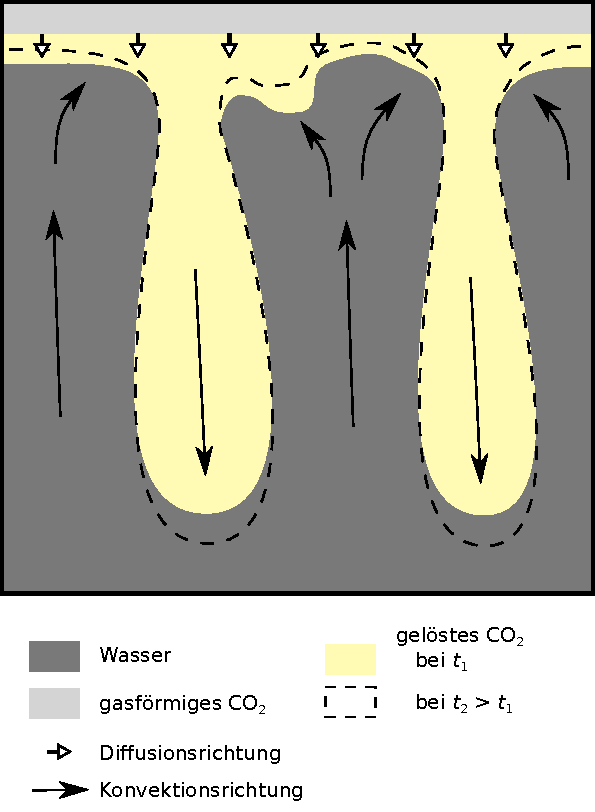
\includegraphics[width=9cm]{./plot/Konvektion_Diffusion.pdf}
%  \caption{Interpretation der auftretenden Phänomene, verursacht durch Konvektion und Diffusion}
%  \label{fig:difkon}
% \end{figure}
% 
% \twocolumn


% \newpage
% \mbox{\,}
\newpage

\section{\COTm Experiment mit porösem Medium}
\label{res:cpm}

\graph[./plot/BCG_test_03_num]{Farbumschläge des \BCG in Verbindung mit verschiedenen Substanzen. \BCG (1) in neutraler Form, \dah im Gleichgewicht mit der umgebenden Luft, (2) in Kombination mit \COT, (3) mit den Glaskügelchen verschiedener Größen, (4) mit Glaskügelchen und gelöstem \COT.}{fig:CPO}

\graph[./plot/BCG_Test_Boro_num]{Farbumschläge des \BCGn. \BCG (1) in neutraler Form, \dah im Gleichgewicht mit der umgebenden Luft, (2) in Kombination mit gelöstem \COT, (3) mit den Glaskügelchen aus \BOG, (4) mit Glaskügelchen und gelöstem \COTn.}{fig:CPO_bor}

Der Versuch das \COTm Experiment in einer mit einem porösen Medium gefüllten \HSC durchzuführen ist aufgrund der hierfür verwendeten Glaskugeln gescheitert. Wasser wird durch einen von Glas induzierten Ionenaustausch basisch. Die leicht löslichen Elemente an der Oberfläche des Glases werden vom Wasser herausgelöst und durch die im Wasser vorhandenen H$^+$-Ionen ersetzt. Dadurch wird das Wasser basisch, da die OH$^-$-Konzentration steigt \citep{Vogel}.

Aufgrund der großen Oberfläche, die die Glaskügelchen durch ihre geringe Größe insgesamt haben, ist dieser Effekt nicht zu vernachlässigen. Er sorgt dafür, dass der benutze Indikator nur den basischen Farbton annimmt. Das Lösen von \COT im Wasser kann diesen Effekt offensichtlich nicht überwiegen.

In Abbildung \ref{fig:CPO} sind die Phänomene veranschaulicht. Man kann erkennen, dass der Indikator einwandfrei das gelöste \COT anzeigt, solange keine Kügelchen mit im Behälter sind. Befinden sich hingegen Glaskügelchen im Behälter, findet auch bei Zugabe von \COT kein Farbumschlag statt.

Ein angedachter Lösungsansatz mit Glaskugeln, welche dem Wasser gegenüber beständiger sind, konnte im Rahmen dieser Arbeit nicht mehr umgesetzt werden. Wie man in Abbildung \ref{fig:CPO_bor} sehen kann ergab ein Test mit Kugeln aus Borosilikatglas aber vielversprechende Ergebnisse, da der durch das \COT hervorgerufene Farbumschlag auch mit Kugeln in der Indikatorlösung beobachtet werden konnte.


% \vspace{10cm} % damit balance die Bilder beide auf die Seite packt



  
% ========================= longgraphpages =========================
\longgraphpage[./plot/plots_data-1/plot_all_overview_quot_0_scale.eps]{Fingerbildung im \COTm Experiment (1/2). Die Farbskala beschreibt die relative Absorption in Bezug auf den Hintergrund. Maximale Absorption bekommt den Wert 100 (rot) zugewiesen, minimale den Wert 0 (blau).}{fig:vcot_1-1}
\longgraphpage[./plot/plots_data-1/plot_all_overview_quot_1_scale.eps]{Fingerbildung im \COTm Experiment (2/2). Die Farbskala beschreibt die relative Absorption in Bezug auf den Hintergrund. Maximale Absorption bekommt den Wert 100 (rot) zugewiesen, minimale den Wert 0 (blau).}{fig:vcot_1-2}

\longgraphpage[./plot/plots_data-1/finger_detection_cut_scale.eps]{Abgebildet ist die Fingerbildung zusammen mit den detektierten Fingerpositionen und -längen zur Demonstration, wie die in Teil \ref{sec:lan} beschriebene Methode funktioniert. Die Farbskala beschreibt die relative Absorption in Bezug auf den Hintergrund. Maximale Absorption bekommt den Wert 100 (rot) zugewiesen, minimale den Wert 0 (blau).}{fig:f_detect}


\longgraphpage[./plot/plots_data-1/plot_all_overview_0_adj_scale]{Fingerbildung im \COTm Experiment. Rohaufnahmen mit erhöhtem Kontrast. Zu erkennen ist der Übergang vom diffusiven zum konvektiven Prozess bei ca. \SI{9}{\minute}. Auch kann man beobachten, wie die diffusive Schicht zwischen den Fingern ``abgesaugt'' wird. }{fig:vcot_1-grey}
% ========================= einzelner Finger =========================
\longgraphpagetriple{./plot/plots_data-1/single_evolution_1}{./plot/plots_data-1/single_evolution_2}{./plot/plots_data-1/single_evolution_3}{Entwicklung eines einzelnen Fingers mit der Zeit. Rohaufnahmen mit erhöhtem Kontrast. Zu erkennen ist der Übergang vom diffusiven zum konvektiven Prozess bei ca. \SI{9}{\minute}, sowie das Dünnerwerden der diffusiven Schicht rechts und links vom Finger im Zeitraum zwischen \SI{9}{\minute} und \SI{24}{\minute}. Dieser Effekt ist in einem Zeitschritt mit roten Kreisen hervorgehoben worden.}{fig:sevo}

\longgraphpagesextuple{./plot/plots_data-1/comp_evolution_1}{./plot/plots_data-1/comp_evolution_2}{./plot/plots_data-1/comp_evolution_3}{./plot/plots_data-1/comp_evolution_4}{./plot/plots_data-1/comp_evolution_5}{./plot/plots_data-1/comp_evolution_6}{Überblick über den gesamten Verlauf des Experiments. Zu erkennen sind die beiden letzten Phasen in die sich der Verlauf des Experiments gliedert: stabile Fingerbildung und die Ausbildung von Vortizitäten, die für Durchmischung der Zelle sorgen. Die Phase, in der sich die diffusive Schicht ausbildet ist zu kurz, als dass sie bei dieser Zeitauflösung zu erkennen wäre. Sie kann in Abbildung \ref{fig:vcot_1-grey} beobachtet werden.}{fig:complete}
% \widegraphpage[./plot/plots_data-1/fingers_quot-raw_5-30_cut.png]{Vergleich der Quotientenmethode und dem tatsächlich aufgezeichneten Bild.}{fig:fing_comp}
